\chapter{Human Tissue}

\section{Introduction}


\section{Methods}

\subsection{Potting}

The geometry of human lumbar vertebrae varies considerably to that of the bovine tail vertebrae from which this methodology is based.
This is characterised by much larger posterior elements with the facets extending much lower, below the bottom of the vertebral body.
Hence, to correctly pot the human vertebrae much more cement must be used, especially for the posterior end-cap, in order to cover the bottom of the vertebral body and the extending posterior elements.
This means that much more of the posterior elements are constrained, therefore restricting the rotation of the vertebral body endplates under axial load.
In addition to this the larger posterior elements which are captured within the PMMA end-caps will transmit load and take a greater share of the load when compared to the bovine tail vertebrae.
Given that vertebroplasty attempts to restore the stiffness of the vertebral body and that there is no understanding of specifically how the loads are shared between the vertebral body and posterior element, this presents a problem.

A solution to this is to remove the posterior elements, following such methods as \cite{Wijayathunga2008,RobsonBrown2014}, where only the vertebral body is modelled.
This allows the stiffness of the vertebral body alone to be captured and modelled.
The posterior elements were removed by cutting through the pedicles at the narrowest part, limiting damage to the region.

To pot the specimens that now lack a spinal canal, a retort stand was used to hold the vertebra, ensuring that both endplates were level on average.
The specimen was then lowered down into the potting container leaving 5 mm between the bottom of the vertebra and the container.
PMMA was poured into the container until the entire of the endplate was touching cement, with the edges of the vertebral body covered.
Care needed to be taken to ensure all of the endplate was in contact with cement, given the extent of osteophytes creating non-flat surfaces in some of the more degenerated specimens.
The other side of the vertebra was potted in a similar manner, however, due to the constraints of the potting container a measured quantity of cement was poured prior to lowering the vertebra into it.
A spirit level ensured parallel end-caps.

\subsection{Loading}

Following previous studies \cite{Wijayathunga2008}, the vertebrae were loaded with an initial maximum load of 800 N for similarly osteoporotic vertebrae.
However, after loading two of the initial set of vertebrae the stiffness continued to increase up to maximum 800 N.
Following loads up to 2000 N showed that the stiffness reached a maximum between 1300 and 2000 N, with three of the initial four specimens showing some degree of failure in the final 400 N of loading.

\subsubsection{Maximum Stiffness Measurement}

The maximum stiffness of the vertebra was found in the same fashion as with the bovine tail vertebrae - measuring the stiffness of segments at increments over the length of the curve.
Given that damage, especially for the intact specimens, needs to be avoided the maximum loads used are on the conservative side.
This can mean that the maximum stiffness is potentially at the end of the dataset or that the stiffness is still increasing at the load cut off.
The solution to the latter would require a prediction of the yield point prior to experimental loading (discussed in Section \ref{predYield}), while the former could potentially be solved by using smaller segment sizes when measuring the stiffness from load - displacement results.

To allow the effect of segment size (the length of each section from which the stiffness is found) and increment size (the size of each increment defining the start point of each segment), the maximum stiffness finding Matlab code was rewritten in Python.
This function could then be iterated over, reporting the maximum stiffness when using an increment size of between 1 and 100 data points (the distance between two data points corresponds to 0.0017 mm).
Changing the increment size becomes a verification of the results using an increment size of 1 data point, given that the only negative of using the smallest possible increment size is computational cost, which is negligible here.

\begin{figure}[ht!]
\centering
\includegraphics[width=6in]{Chapters/Chapter_HT_images/findStiffness_1incr.png}
\caption{The effect of reducing the segment size on the maximum stiffness reported from four human vertebrae loaded to 2000 N pre and post augmentation. Using an increment size of 1 data point (0.0017 mm) and segment sizes of 100 to 1 data point (0.17 mm to 0.0017 mm).}
\label{fig:findStiffness_1incr}
\end{figure}

\begin{figure}[ht!]
\centering
\includegraphics[width=6in]{Chapters/Chapter_HT_images/findStiffness_20incr.png}
\caption{The effect of reducing the segment size on the maximum stiffness reported from four human vertebrae loaded to 2000 N pre and post augmentation. Using an increment size of 20 data points (0.0037 mm) and segment sizes of 100 to 1 data point (0.17 mm to 0.0017 mm).}
\label{fig:findStiffness_20incr}
\end{figure}

Using an increment size of 1 data points width, as shown in Figure \ref{fig:findStiffness_1incr} shows a smaller variation across the range of segment sizes compared to using 20 points in Figure \ref{fig:findStiffness_20incr}.
The effect of both segment size and increment size is especially evident for the two G19-11 L1 vertebrae both intact and post augmentation where the stiffness continues to increase until the end of the test at 2000 N.
Meaning that there is a much smaller linear region for these two specimens, hence requiring a smaller segment size to measure the largest gradient.

Choosing values for the segment size to use moving forwards becomes difficult given the large effect it can have on the measured maximum stiffness (a range of over 1000 N/mm in the case the two G19-11 L1 tests).
The segment size needs to be small enough to capture the maximum stiffness while avoiding the noise when using a segment size below 18 data points.
Hence, a value of 20 data points was chosen, a value that avoids the noise while being on the plateau of the lines.


\subsubsection{Repeated Loading}

Given the nature of the test, attempting to limit damage to the vertebrae, especially during their initial intact load, the ability to derive errors becomes difficult especially from a single load.
To attempt to understand this error four vertebrae having undergone augmentation were tested three more times in an iterative fashion, removing each from the load testing machine, testing the next specimen in the set and repeating.
Removing the vertebrae from their steel housing (instead of three tests while seated in the steel housing) allowed the error in loading position and setup to be tested along with repeated loading of the vertebrae to be tested.

The results of repeated loading can be seen in Figure \ref{fig:exp_repeats}.
All four specimens show a reduced stiffness for the repeated loads following the initial load, for which there are two possible reasons.
One possibility for the reduction in stiffness is that it is a consequence of the freeze thaw cycle that occurred between these tests.
The second possibility is that the vertebrae were still partially frozen while the testing took place.
The frozen bar in Figure \ref{fig:exp_repeats} shows how the stiffness increases when the vertebrae are completely frozen, potentially helping to explain the drop in stiffness found in the repeats.
Further tests will be carried out with three more repeats following another freeze thaw cycle to attempt to answer this.

The iterative reduction in stiffness for the G21-11 L2 vertebrae can be explained as damage being caused after each iteration.
This can be seen in Figure \ref{fig:G21-11_L2}, with the three repeats each showing a yielding before the 1600 N limit and a smaller maximum load and stiffness after each repeat.

Figures \ref{fig:G19-11_L1} through to \ref{fig:G21-11_L3} show the data for the loading, from which the maximum stiffness values are found.
This excludes the initial cyclic loading, starts the loading at 50 N and displacement at 0 mm.

\begin{figure}[!h]
\centering
\includegraphics[width=6in]{Chapters/Chapter_HT_images/experimental_repeats.png}
\caption{The stiffness of four augmented vertebral specimens over the course of an initial load, three repeated loads and a load while frozen. The intact specimen was loaded until 2000 N while the remaining four were loaded until 1600 N.}
\label{fig:exp_repeats}
\end{figure}


\begin{figure}[H]
\centering
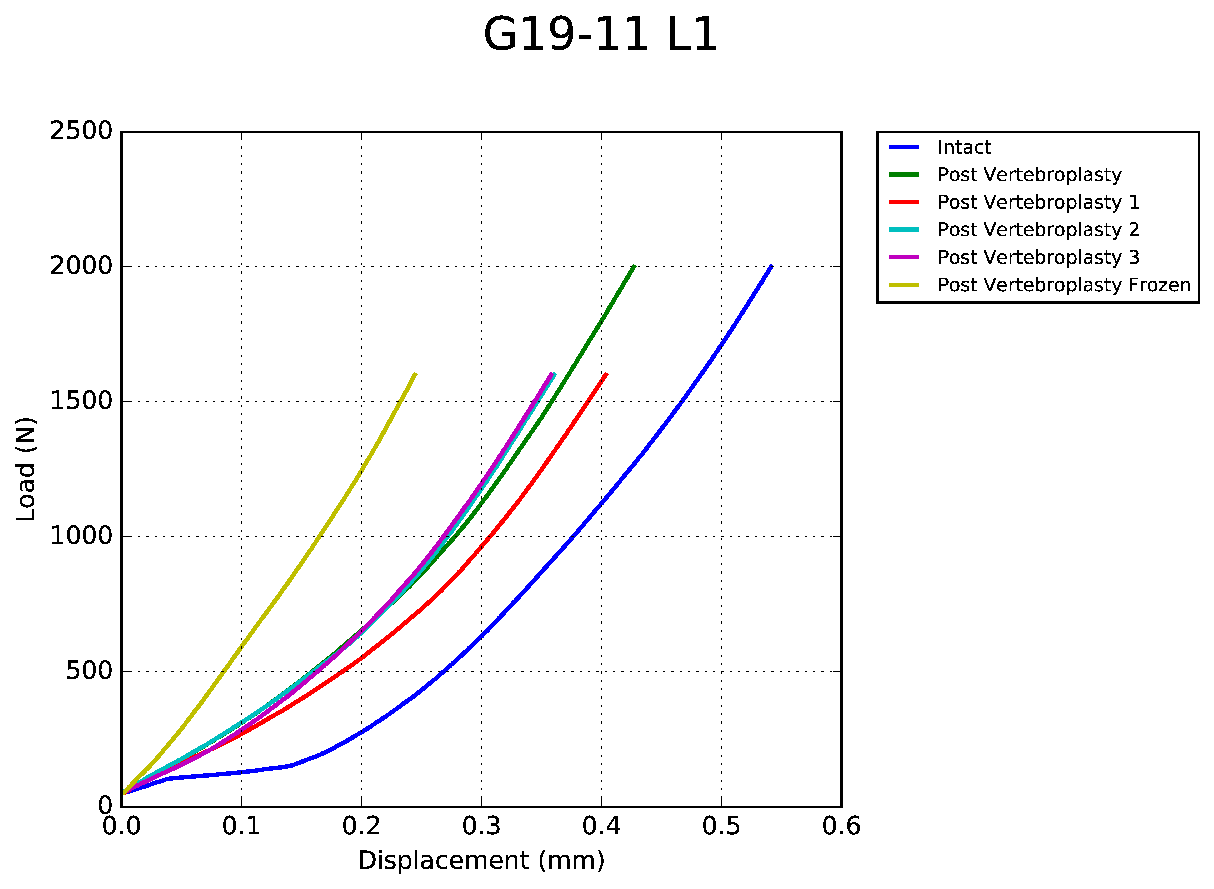
\includegraphics[width=4in]{Chapters/Chapter_HT_images/G19-11_L1.pdf}
\caption{The load - displacement results for the G19-11 L1 vertebra. Showing results of the intact load and post augmentation load up to 2000 N and the repeats and frozen load up to 1600 N.}
\label{fig:G19-11_L1}
\end{figure}

\begin{figure}[H]
\centering
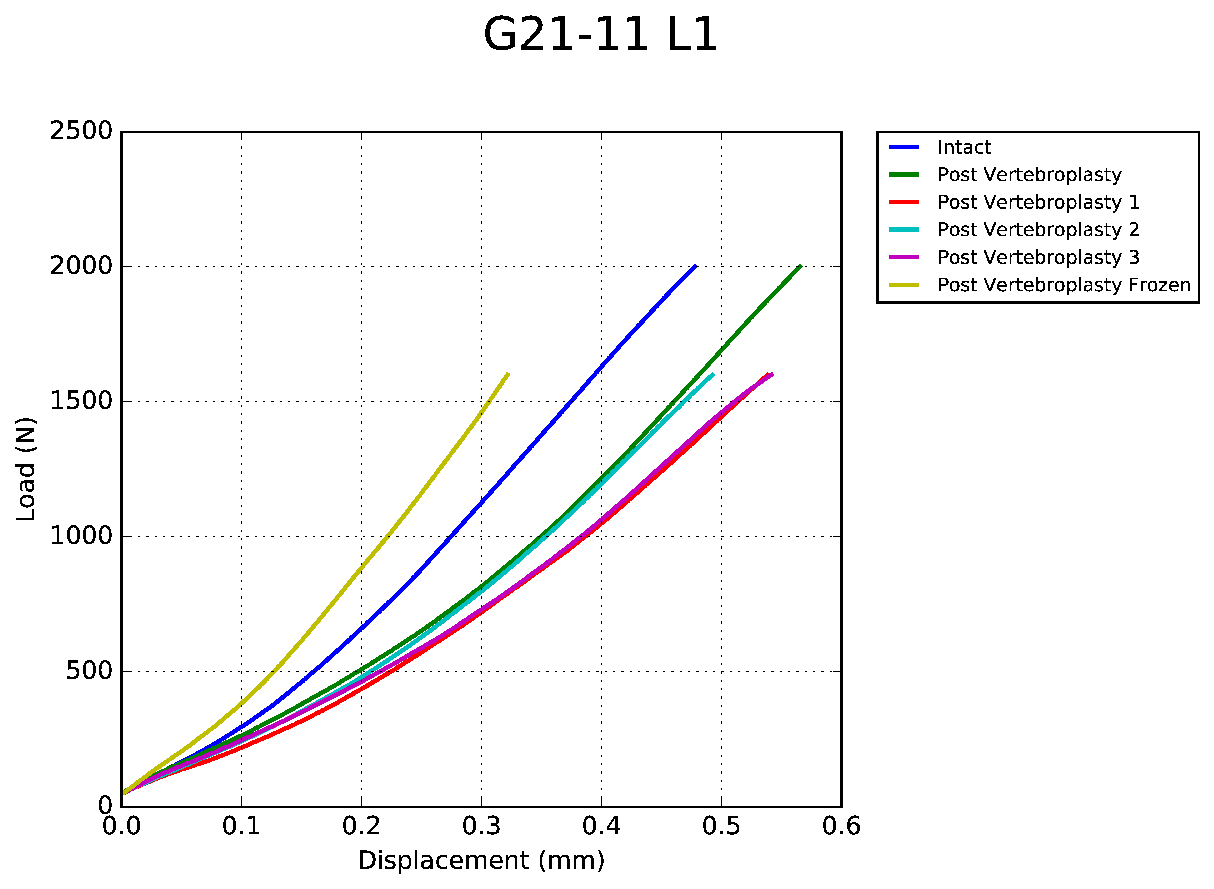
\includegraphics[width=4in]{Chapters/Chapter_HT_images/G21-11_L1.pdf}
\caption{The load - displacement results for the G21-11 L1 vertebra. Showing results of the intact load and post augmentation load up to 2000 N and the repeats and frozen load up to 1600 N.}
\label{fig:G21-11_L1}
\end{figure}

\begin{figure}[H]
\centering
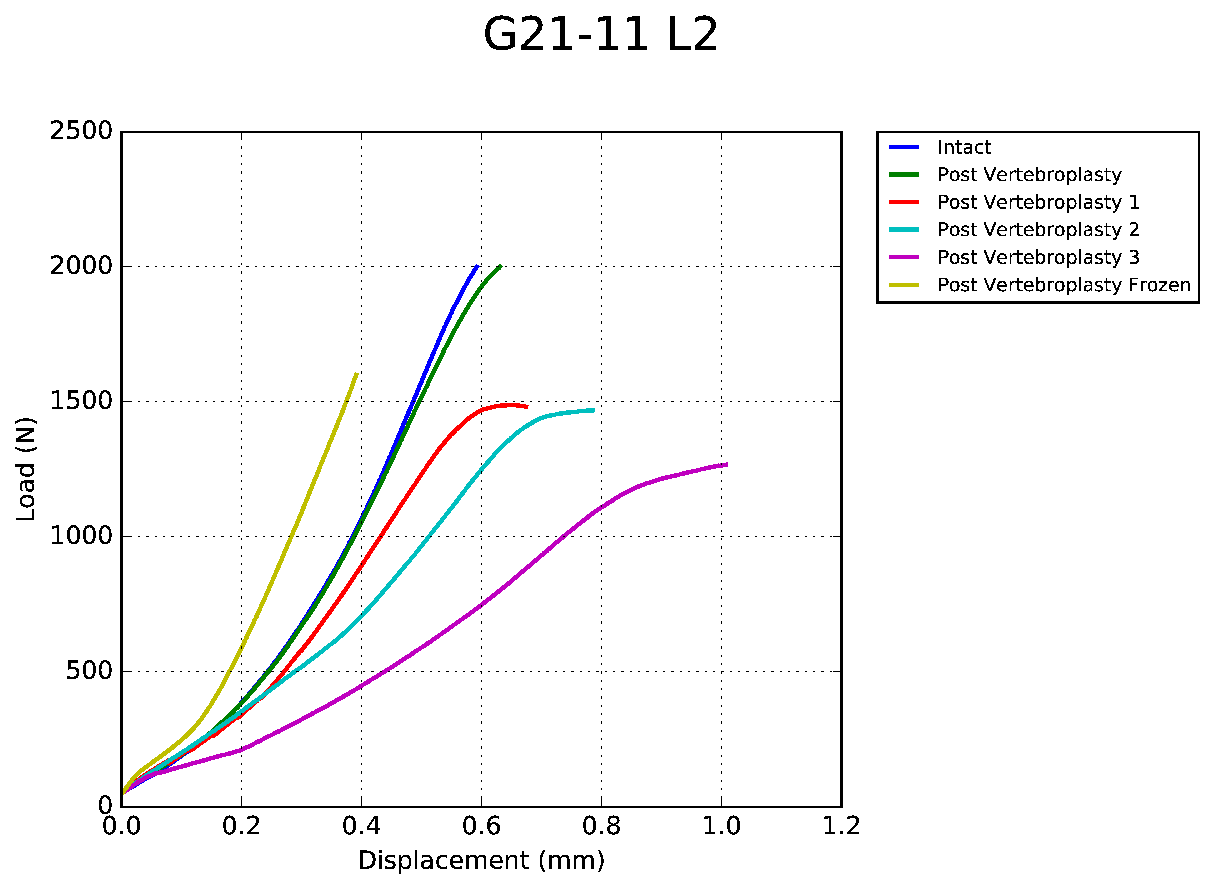
\includegraphics[width=4in]{Chapters/Chapter_HT_images/G21-11_L2.pdf}
\caption{The load - displacement results for the G21-11 L2 vertebra. Showing results of the intact load and post augmentation load up to 2000 N and the repeats and frozen load up to 1600 N.}
\label{fig:G21-11_L2}
\end{figure}

\begin{figure}[H]
\centering
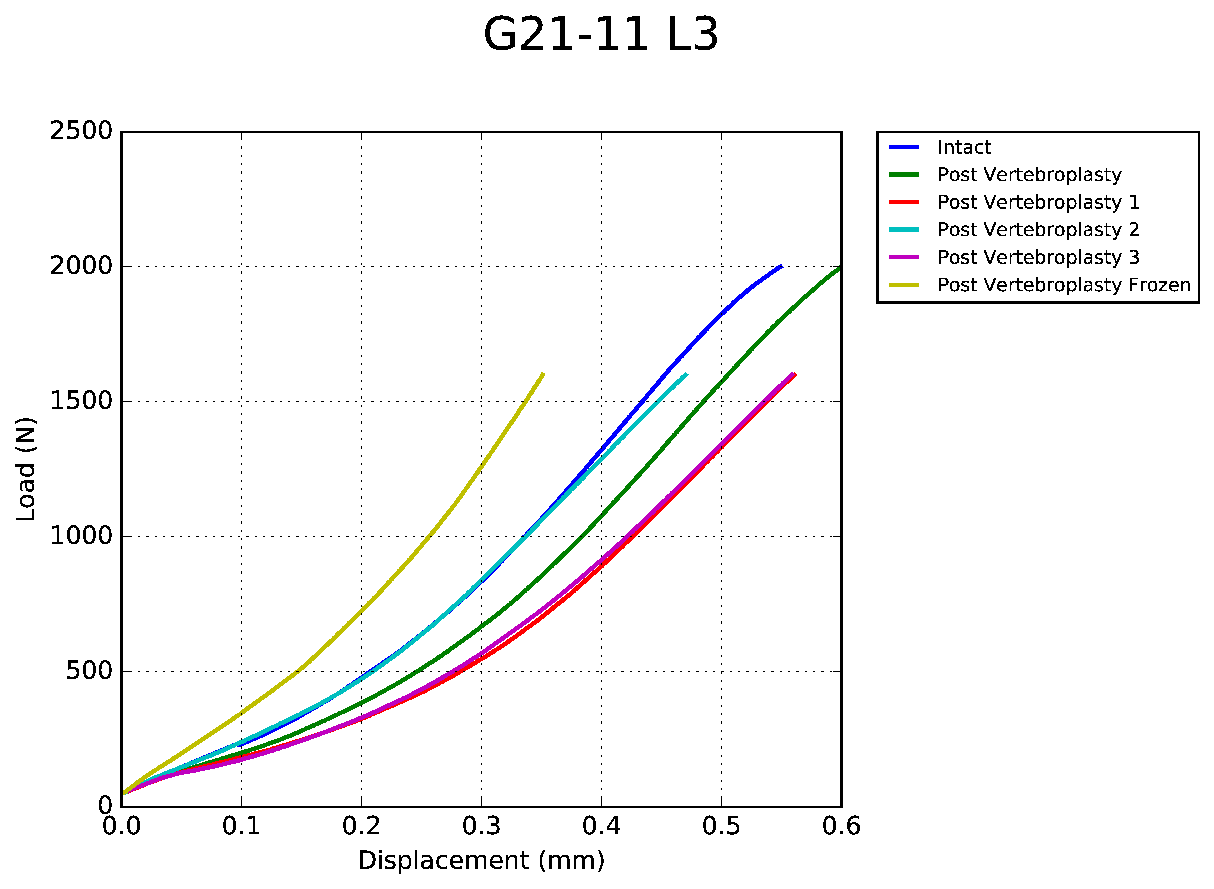
\includegraphics[width=4in]{Chapters/Chapter_HT_images/G21-11_L3.pdf}
\caption{The load - displacement results for the G21-11 L3 vertebra. Showing results of the intact load and post augmentation load up to 2000 N and the repeats and frozen load up to 1600 N.}
\label{fig:G21-11_L3}
\end{figure}






\subsection{Vertebroplasty}

Despite the development of methods for the augmentation of bovine tail vertebrae, the methods for augmenting human vertebrae were altered due to the different geometry and density.
The human vertebrae, being much less dense, did not require the vertebroplasty needle to be inserted with the aid of a mallet.
Instead the needle could be pushed by hand through the cortical shell and into the vertebral body.

An additional difference was the approach with the needle, instead of entering the vertebrae through their pedicles an oblique approach was adopted.
This was due to variation in pedicle diameter between the L1 - L5 lumbar levels and therefore the potential to damage the region and its load sharing capabilities.
The oblique approach therefore avoided creating this damage to the pedicle-canal region, especially for the vertebrae with narrower pedicles and instead created much less damage to the vertebral body.

A final difference to the needle insertion methods was a change to the needle.
Here, a side opening needle was used, allowing the cement to be directed into the anterior-centre region of the vertebral body as opposed to directly out of the needle end.

Quantity?


\subsection{Modelling}

\subsubsection{Predicting Vertebral Yield Point}\label{predYield}

\subsubsection{Load Position Sensitivity}


\subsubsection{--}

\section{Results}

\section{Discussion}

\section{Conclusion}







